\documentclass[12pt]{article}

\usepackage[parfill]{parskip}
\usepackage{fancyhdr}
\usepackage[fleqn]{amsmath}
\usepackage{amssymb}
\usepackage{hyperref}
\usepackage{enumitem}
\usepackage{tikz}

\pagestyle{fancy}
\fancyhf{}
\setlength{\headheight}{15pt}
\lhead{\textbf{MAU22C00} Discrete Mathematics}
\rhead{Ted Johnson ‑ 19335618}
\rfoot{\thepage}

\newcommand{\qedsymbol}{\rule{0.7em}{0.7em}}
\def\<#1>{\langle\ignorespaces#1\unskip\rangle}

\urlstyle{same}
\hypersetup{colorlinks=true, linkcolor=blue, urlcolor=blue}

\usetikzlibrary{automata,positioning}
\tikzset{->,node distance=3cm,every state/.style={thick, fill=gray!20}}

\begin{document}

\section*{Assignment 3}

I have read and I understand the plagiarism provisions in the General Regulations of the University Calendar for the current year, found at \href{http://www.tcd.ie/calendar}{here}.
I have also completed the Online Tutorial on avoiding plagiarism ‘Ready Steady Write’, located \href{http://tcd-ie.libguides.com/plagiarism/ready-steady-write}{here}.

\subsection*{Exercise 1}

(40 points) Let $L$ be the language over the alphabet $A=\{\,0,1\,\}$ consisting of all words containing an even number of zeroes.

\subsubsection*{Part (a)}

Draw a finite state acceptor that accepts the language $L$.
Carefully label all the states including the starting state and the finishing states as well as all the transitions.
Make sure you justify it accepts all strings in the language $L$ and no others.

\subsubsection*{Solution}

The finite state acceptor should be left in an accepting state only if it has received an even number of zeros.
To model this, we need only two states:

\begin{figure}[ht]
	\centering
	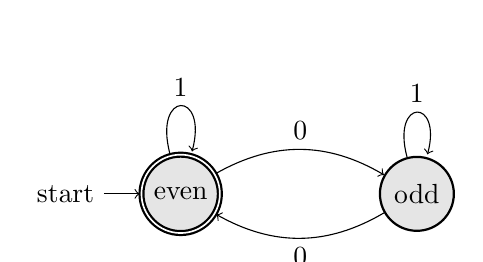
\begin{tikzpicture}
		\node[state, initial, accepting] (e) {even};
		\node[state, right of = e]       (o) {odd};
		\path[->]
			(e) edge[loop above]       node {1} (e)
			(e) edge[bend left, above] node {0} (o)
			(o) edge[loop above]       node {1} (o)
			(o) edge[bend left, below] node {0} (e);
	\end{tikzpicture}
\end{figure}

Initially, the finite state acceptor is in the \textit{even} state, as there have been zero 0 characters received.
It stays in the \textit{even} state until a 0 character is received.
After the first 0 character, the internal state transitions to \textit{odd}.
Again, it stays in this state until a subsequent 0 character is passed to it, which returns the internal state to \textit{even} again.
The string is only accepted if the internal state finishes on the \textit{even} state.

In this way, only strings with an even number of 0 characters leave the internal state as \textit{even}, thus only these strings are accepted for the language $L$.

\subsubsection*{Part (b)}

Devise a regular grammar in normal form that generates the language $L$.
Be sure to specify the start symbol, the non-terminals and all the production rules.

\subsubsection*{Solution}

The initial state of the finite state acceptor is the $\<E>$ state.
This is also the only accepting state.
It has three production rules for transitioning:
\begin{enumerate}[label = (\arabic*)]
	\item $\<E> \rightarrow 1\<E>$
	\item $\<E> \rightarrow 0\<O>$
	\item $\<E> \rightarrow \epsilon$
\end{enumerate}
On receiving a 1 character, the acceptor remains in the $\<E>$ state: The number of 0 characters received has not changed.
On receiving a 0 character, the acceptor transitions to the $\<O>$ state: The number of 0 characters received has increased by one, from an even number to an odd number, taking the acceptor out of an accepting state.
Finally, as this is an accepting state, it also has a production rule of type (iii).

The only other state is when the acceptor has so far received an odd number of 0 characters, labeled the $\<O>$ state.
It has two production rules for transitioning:
\begin{enumerate}[label = (\arabic*), resume]
	\item $\<O> \rightarrow 1\<O>$
	\item $\<O> \rightarrow 0\<E>$
\end{enumerate}
On receiving a 1 character, the acceptor remains in the $\<O>$ state: The number of 0 characters received has not changed.
On receiving a 0 character, the acceptor transitions back to the $\<E>$ state: The number of 0 characters received has again increased by one, now from an odd number to an even number, returning the acceptor to an accepting state.

\pagebreak
\subsubsection*{Part (c)}

Write down a regular expression that gives the language $L$ and justify.

\subsubsection*{Solution}

A regular expression that matches only language $L$ would be ${(1 \cup 01^{*}0)}^{*}$.
To understand this expression, we will break it down into its components:

The inner expression $1 \cup 01^{*}0$ accepts either a single 1 character or two 0 characters separated by an arbitrary number of 1 characters.
Recalling the finite state acceptor diagram, this expression insures that the internal state of the acceptor either remains in the $even$ state or transitions to the $odd$ state and then returns to the $even$ state again.

Wrapping this expression in a Kleene star allows this pattern to repeat. This covers all words in $L$.

\subsubsection*{Part (d)}

Prove that language $L$ is regular from the definition.

\subsubsection*{Solution}

To prove $L$ is a regular language, we must show that a finite sequence $L_{1}, L_{2}, \ldots, L_{m}$ exists where $L = L_m$ and $\forall i,\ 1 \leq i \leq m,\ L_{i}$ satisfies one:
\begin{enumerate}[label = \arabic*.]
	\item $L_{i}$ is a finite set.
	\item $L_{i} = L_{j}^{*}$ where $1 \leq j \leq i$.
	\item $L_{i} = L_{j} \circ L_{k}$ where $1 \leq j,k \leq i$.
	\item $L_{i} = L_{j} \cup L_{k}$ where $1 \leq j,k \leq i$.
\end{enumerate}

As shown before, $L$ can be given by ${(1 \cup 01^{*}0)}^{*}$. $L$ is regular if ${(1 \cup 01^{*}0)}^{*}$ can be shown to give a regular language using the rules above.

$0 1^{*} 0$ gives a regular language, as $1^{*}$ follows the second property and $0 \circ 1^{*} \circ 0$ simply concatenates finite sets which combines the first and third properties.
Then $1 \cup 0 1^{*} 0$ must give a regular language, as $1$ is a finite set and $1 \cup 0 1^{*} 0$ follows from the fourth property.
With this, ${(1 \cup 01^{*}0)}^{*}$ must give a regular language through applying the second property to $1 \cup 0 1^{*} 0$.

\pagebreak

\subsection*{Exercise 2}

(20 points) Let $M$ be the language over the alphabet $\{\,a, r, c\,\}$ given by \sloppy${M=\{\,a^{i}r^{j}c^{k} \mid i,j,k \ge 0 \land i = 2j - k\,\}}$.

\subsubsection*{Part (a)}

Use the Pumping Lemma to show this language is not regular.

\subsubsection*{Solution}

Assuming language $M$ is regular, then it must have a pumping length $p$.
Therefore all strings in $M$ longer than $p$ must satisfy the pumping conditions.

Consider a word $w = a^{p} r^{j} c^{k}$. Clearly, $|w| \geq p$. For $w$ to also be a word in $M$, then $p = 2j - k$.
As $w$ is a string in $M$ longer than $p$, it must satisfy the pumping conditions.

Suppose $w$ can be split up so that $w = xuy$. According to the pumping conditions, $|xu| \leq p$ and $|u| > 0$.
Therefore, $xu = a^{+}$ as the $a$ substring of $w$ has a length of $p$. Clearly, $u = a^{+}$ as well.
Then $y$ must equal the remaining $a^{*}r^{j} c^{k}$.

But if that is the case, the pumping condition $\forall i\ xu^{i}y \in M$ could not hold.
Changing the value of $i$ would result in a different length of $a$ symbols in the string.
This does not follow the requirements of language $M$ that $i = 2j - k$ where $a^{i} r^{j} c^{k} \in M$.
Therefore, language $M$ does not have the pumping property and, as such, is not a regular language.

\subsubsection*{Part (b)}

Write down the production rules of a context-free grammar that generates exactly $M$ and justify your answer.

\subsubsection*{Solution}

To design production rules to generate exactly $M$, we must first consider the requirements of the language.
Words in $M$ follow the rule $w = a^{i} r^{j} c^{k}$ where $i = 2j - k$.
If we rearrange this to $2j = i + k$, you can notice that for every $r$ character in a word, there must be two of either of the other characters in the alphabet.

It is helpful to now consider how patterns may form between words in $M$ from this.
To follow the above rule, a word must keep this equation `balanced'.
If another $r$ character is added, a combination of two $a$ and $c$ characters must be added to compensate.
To capture this behaviour in context-free grammar, we will split the additional $r$ characters added between prepending or appending to the previously added $r$ characters.
This allows us to compensate for the $r$ character with two equal characters.

To do this, the starting symbol $\<S>$ is split into two recursive symbols, $\<A>$ and $\<C>$.
The $\<A>$ symbol continuously prepends two $a$ characters to a prepended $r$.
The $\<C>$ symbol continuously appends two $c$ characters to an appended $r$.
As we compensate each $r$ character with two alternative characters, we must add an additional production rule to cover when there are an odd number of $a$ and $c$ characters.
\begin{enumerate}[label = (\arabic*)]
	\item $ \<S> \rightarrow \<A> \<C> $
	\item $ \<S> \rightarrow a \<A> r \<C> c $
\end{enumerate}

These recursive symbols work by either continuing the chain or inserting an empty string.
\begin{enumerate}[label = (\arabic*), resume]
	\item $ \<A> \rightarrow a a \<A> r $
	\item $ \<A> \rightarrow \epsilon $
	\item $ \<C> \rightarrow r \<C> c c $
	\item $ \<C> \rightarrow \epsilon $
\end{enumerate}

These six production rules cover the language $M$.
Any number of $aa\<A>r$ or $r\<C>cc$ iterations does not unbalance $i = 2j - k$.
Additionally, the alternative starting symbol production rule offsets these iterations by the three characters $arc$,
which gives the initially missed words that contain an odd number of $a$ and odd number of $c$ characters.

\end{document}

